\documentclass[A4paper, 12pt, british, reqno]{amsart}

%%% Contents of the preamble
    % Packages ----------------- Line 12
    % General things ----------- Line 72
    % Font definitions --------- Line 87
    % Theorem environments ----- Line 230
    % Tikzcd ------------------- Line 395
    % Author, title, etc ------- Line 416
    % \begin{document} --------- Line 458

%%% Packages

\usepackage{libertine}
\usepackage[libertine]{newtxmath}
% Local font definition; before fontenc, cf. https://tex.stackexchange.com/a/2867

\usepackage[T1]{fontenc}
% This uses 8-bit font encoding (with 256 glyphs) instead of the default 7-bit font encoding (with 128 glyphs). For example, with this option ö is a single glyph in the font, whereas on the 7-bit font encoding the font ö is made by adding an accent to the existing glyph o. A bad consequence of not using this package is that you cannot properly copy-paste such words form the output pdf file. Also, for some reason, funny stuff happens with |, < and > in text.
% Some people suggest to load fontenc before inputenc, most agree that it does not matter.

\usepackage[utf8]{inputenc}
% When you type ä in an editor set up for utf8, the machine stores the character number 228. When TeX reads the file it finds the character number 228 and the macros of inputenc transform this into \"a. Finally fontenc does its thing and transforms this into the command print character 228 (otherwise the two things would be printed separatedly as explained in fontenc).

\usepackage[UKenglish]{babel}
% To manage culturally determined typographical and similar rules, in this case for british english. Some people suggest to load babel after fontenc to avoid warnings, although most agree that it does not matter.

\usepackage{mathtools}
% Loads the amsmath package (\usepackage{amsmath}: miscellaneous improvements such as the commands \DeclareMathOperator and \text). It fixes some quirks it has and adds some useful settings, symbols and environments. It improves the aesthetics as well.

\usepackage{amssymb}
% Extended symbol collection, e.g. \Cap and \Cup. More importantly: the \mathbb command! It loads the amsfonts package (\usepackage{amsfonts}: fraktur letters, bold Greek letters...), so we do not need to include it in the preamble anymore.

\usepackage{mathrsfs}
% Font package (only supports upper case letters).

\usepackage{enumitem}
% To control the layout of enumerate, itemize and description. It supersedes the enumerate package.

\usepackage{tikz-cd}
% To draw commutative diagrams.
\usetikzlibrary{decorations.markings}
% For open and closed immersions.

\usepackage{graphicx}
% An extension of the graphics package, with optional arguments for the \includegraphics command.

\usepackage{todonotes}
% To write to do notes use the command \todo.

\usepackage{xcolor}
% To write in colors.

\usepackage{marginnote}
% To write on margins.

\usepackage{manfnt}
% To draw dangerous bent symbol.

\usepackage{float}
% Improved interface for floating objects such as figures and tables, introducing for example the H modifier to force the position of a float in the page or the boxed float. Should be loaded before hyperref.

\usepackage[backref=page]{hyperref}
% To handle cross-referencing and produce hypertext links in the document. It should be loaded last (with few exceptions), because it redefines many LaTeX commands.
% The backref option inserts links on each bibliography entry to the pages in which the citation was used.
%% The hidelinks option removes colors and boxes around links, but the links remain clickable. On firefox the links are even highlighted when the mouse pointer passes over them.
\renewcommand{\backref}[1]{$\uparrow$~#1}
% Adds an upwards arrow before referencing to the pages in which the citations appear.

\usepackage[noabbrev]{cleveref}
% Enhances cross-referencing features, e.g. to reference to a theorem and automatically include the word theorem.
% No abbreviature option to write figure instead of fig. etc.

%%% General things

% Custom colors
\definecolor{darkgreen}{RGB}{0,75,0}
\definecolor{darkblue}{RGB}{0,0,75}
\definecolor{darkred}{RGB}{75,0,0}
\definecolor{linkred}{rgb}{0.6,0.2,0.2}
\definecolor{linkblue}{rgb}{0,0.2,0.6}
\definecolor{linkgreen}{rgb}{0.2,0.6,0.2}

% Limit table of contents to section titles
\setcounter{tocdepth}{1}

% Sloppy formatting -- often looks better
\sloppy

%%% Font definitions

% Script Font used for sheaves
\DeclareFontFamily{OMS}{rsfs}{\skewchar\font'60}
\DeclareFontShape{OMS}{rsfs}{m}{n}{<-5>rsfs5 <5-7>rsfs7 <7->rsfs10 }{}
\DeclareSymbolFont{rsfs}{OMS}{rsfs}{m}{n}
\DeclareSymbolFontAlphabet{\scr}{rsfs}
\DeclareSymbolFontAlphabet{\scr}{rsfs}

% Sheaves
\newcommand{\sA}{\scr{A}}
\newcommand{\sB}{\scr{B}}
\newcommand{\sC}{\scr{C}}
\newcommand{\sD}{\scr{D}}
\newcommand{\E}{\scr{E}} % Exception (Vector bundles)
\newcommand{\F}{\scr{F}} % Exception (Coherent sheaves)
\newcommand{\G}{\scr{G}} % Exception (Coherent sheaves)
\newcommand{\sH}{\scr{H}}
\renewcommand{\hom}{\scr{H}\negthinspace om} % Exception (Hom-sheaf)
\newcommand{\I}{\scr{I}} % Exception (Ideal sheaves)
\newcommand{\sJ}{\scr{J}}
\newcommand{\sK}{\scr{K}}
\renewcommand{\L}{\scr{L}} % Exception (Line bundles)
\newcommand{\M}{\scr{M}} % Exception (Line bundles)
\newcommand{\sN}{\scr{N}}
\renewcommand{\O}{\scr{O}} % Exception (Structure sheaf)
\newcommand{\sP}{\scr{P}}
\newcommand{\sQ}{\scr{Q}}
\newcommand{\sR}{\scr{R}}
\newcommand{\sS}{\scr{S}}
\newcommand{\sT}{\scr{T}}
\newcommand{\sU}{\scr{U}}
\newcommand{\sV}{\scr{V}}
\newcommand{\sW}{\scr{W}}
\newcommand{\w}{\omega} % Addition (Canonical sheaf)
\newcommand{\sX}{\scr{X}}
\newcommand{\sY}{\scr{Y}}
\newcommand{\sZ}{\scr{Z}}

% Mathcal fonts
\newcommand{\calA}{\mathcal{A}}
\newcommand{\calB}{\mathcal{B}}
\newcommand{\calC}{\mathcal{C}}
\newcommand{\calD}{\mathcal{D}}
\newcommand{\calE}{\mathcal{E}}
\newcommand{\calF}{\mathcal{F}}
\newcommand{\calG}{\mathcal{G}}
\newcommand{\calH}{\mathcal{H}}
\newcommand{\calI}{\mathcal{I}}
\newcommand{\calJ}{\mathcal{J}}
\newcommand{\calK}{\mathcal{K}}
\newcommand{\calL}{\mathcal{L}}
\newcommand{\calM}{\mathcal{M}}
\newcommand{\calN}{\mathcal{N}}
\newcommand{\calO}{\mathcal{O}}
\newcommand{\calP}{\mathcal{P}}
\newcommand{\calQ}{\mathcal{Q}}
\newcommand{\calR}{\mathcal{R}}
\newcommand{\calS}{\mathcal{S}}
\newcommand{\calT}{\mathcal{T}}
\newcommand{\U}{\mathcal{U}} % Exception (Open covers)
\newcommand{\calV}{\mathcal{V}}
\newcommand{\calW}{\mathcal{W}}
\newcommand{\X}{\mathcal{X}} % Exception (Families of varieties)
\newcommand{\Y}{\mathcal{Y}} % Exception (Families of varieties)
\newcommand{\calZ}{\mathcal{Z}}

% Blackboard Bold Symbols
\newcommand{\A}{\mathbb{A}} % Exception (Affine space)
\newcommand{\bbB}{\mathbb{B}}
\newcommand{\C}{\mathbb{C}} % Exception (Complex numbers)
\newcommand{\bbD}{\mathbb{D}}
\newcommand{\bbE}{\mathbb{E}}
\newcommand{\bbF}{\mathbb{F}}
\newcommand{\bbG}{\mathbb{G}}
\newcommand{\Gm}{\mathbb{G}_{\mathrm{m}}} % Addition (Punctured affine line)
\newcommand{\bbH}{\mathbb{H}}
\newcommand{\bbI}{\mathbb{I}}
\newcommand{\bbJ}{\mathbb{J}}
\newcommand{\bbK}{\mathbb{K}}
\newcommand{\bbL}{\mathbb{L}}
\newcommand{\bbM}{\mathbb{M}}
\newcommand{\N}{\mathbb{N}} % Exception (Natural numbers)
\newcommand{\bbO}{\mathbb{O}}
\renewcommand{\P}{\mathbb{P}} % Exception (Projective space)
\newcommand{\Q}{\mathbb{Q}} % Exception (Rational numbers)
\newcommand{\R}{\mathbb{R}} % Exception (Real numbers)
\newcommand{\bbS}{\mathbb{S}}
\newcommand{\bbT}{\mathbb{T}}
\newcommand{\bbU}{\mathbb{U}}
\newcommand{\V}{\mathbb{V}} % Exception (Geometric vector bundle)
\newcommand{\bbW}{\mathbb{W}}
\newcommand{\bbX}{\mathbb{X}}
\newcommand{\bbY}{\mathbb{Y}}
\newcommand{\Z}{\mathbb{Z}} % Exception (Integers)

% Boldfont (categories)
\newcommand{\bfA}{\mathbf{A}}
\newcommand{\Ab}{\mathbf{Ab}}
\newcommand{\bfB}{\mathbf{B}}
\newcommand{\bfC}{\mathbf{C}}
\newcommand{\Cat}{\mathbf{Cat}} % Addition (Categories)
\newcommand{\Coh}{\mathbf{Coh}} % Addition (Coherent sheaves)
\newcommand{\D}{\mathbf{D}} % Exception (Derived category)
\newcommand{\Db}{\mathbf{D}^{\mathrm{b}}} % Addition (Bounded derived category)
\newcommand{\bfE}{\mathbf{E}}
\newcommand{\bfF}{\mathbf{F}}
\newcommand{\bfG}{\mathbf{G}}
\newcommand{\bfH}{\mathbf{H}}
\newcommand{\bfI}{\mathbf{I}}
\newcommand{\bfJ}{\mathbf{J}}
\newcommand{\K}{\mathbf{K}} % Exception (Homotopy category)
\newcommand{\bfL}{\mathbf{L}}
\newcommand{\bfM}{\mathbf{M}}
\newcommand{\Mod}{\mathbf{Mod}} % Addition (Modules)
\newcommand{\bfN}{\mathbf{N}}
\newcommand{\bfO}{\mathbf{O}}
\newcommand{\bfP}{\mathbf{P}}
\newcommand{\PSh}{\mathbf{PSh}} % Addition (Presheaves)
\newcommand{\bfQ}{\mathbf{Q}}
\newcommand{\QCoh}{\mathbf{QCoh}} % Addition (Quasi-coherent sheaves)
\newcommand{\bfR}{\mathbf{R}}
\newcommand{\bfS}{\mathbf{S}}
\newcommand{\Set}{\mathbf{Set}} % Addition (Sets)
\newcommand{\Sh}{\mathbf{Sh}} % Addition (Sheaves)
\newcommand{\bfT}{\mathbf{T}}
\newcommand{\bfU}{\mathbf{U}}
\newcommand{\bfV}{\mathbf{V}}
\renewcommand{\Vec}{\mathbf{Vec}} % Addition (Vector bundles)
\newcommand{\bfW}{\mathbf{W}}
\newcommand{\bfX}{\mathbf{X}}
\newcommand{\bfY}{\mathbf{Y}}
\newcommand{\bfZ}{\mathbf{Z}}

% Mathfrak for ideals
\renewcommand{\a}{\mathfrak{a}}
\renewcommand{\b}{\mathfrak{b}}
\renewcommand{\c}{\mathfrak{c}}
\renewcommand{\d}{\mathfrak{d}}
\newcommand{\e}{\mathfrak{e}}
\newcommand{\m}{\mathfrak{m}}
\newcommand{\n}{\mathfrak{n}}

%%% Theorem environments

% Custom theorem styles (empty fields take default values)
\newtheoremstyle{darkgreentheorem}% name of the style
{}% measure of space to leave above the theorem. E.g.: 3pt
{}% measure of space to leave below the theorem. E.g.: 3pt
{\itshape}% name of font to use in the body of the theorem
{}% measure of space to indent
{\color{darkgreen}\bfseries}% name of head font
{.}% punctuation between head and body
{ }% space after theorem head; " " = normal interword space
{}% Manually specify head
\newtheoremstyle{darkbluedefinition}
{}{}{}{}{\color{darkblue}\bfseries}{.}{ }{}
\newtheoremstyle{darkredexample}
{}{}{}{}{\color{darkred}\bfseries}{.}{ }{}

% Numbered theorems
\theoremstyle{plain}
% \theoremstyle{darkgreentheorem}
\newtheorem{thm}{Theorem}[section]
\newtheorem{lm}[thm]{Lemma}
\newtheorem{prop}[thm]{Proposition}
\newtheorem{cor}[thm]{Corollary}
\newtheorem{conj}[thm]{Conjecture}
\newtheorem{fact}[thm]{Fact}
\theoremstyle{definition}
% \theoremstyle{darkbluedefinition}
\newtheorem{defn}[thm]{Definition}
% \theoremstyle{darkredexample}
\newtheorem{exa}[thm]{Example}
\theoremstyle{remark}
\newtheorem{rem}[thm]{Remark}
\newtheorem{nota}[thm]{Notation}
\newtheorem{q}[thm]{Question}
\newtheorem{exe}[thm]{Exercise}

% Custom numbered theorems
\theoremstyle{plain}
% \theoremstyle{darkgreentheorem}
\newtheorem{innercustomthm}{Theorem}
\newenvironment{cthm}[1]
    {\renewcommand\theinnercustomthm{#1}\innercustomthm}
    {\endinnercustomthm}
\newtheorem{innercustomlm}{Lemma}
\newenvironment{clm}[1]
    {\renewcommand\theinnercustomlm{#1}\innercustomlm}
    {\endinnercustomlm}
\newtheorem{innercustomprop}{Proposition}
\newenvironment{cprop}[1]
    {\renewcommand\theinnercustomprop{#1}\innercustomprop}
    {\endinnercustomprop}
\newtheorem{innercustomcor}{Corollary}
\newenvironment{ccor}[1]
    {\renewcommand\theinnercustomcor{#1}\innercustomcor}
    {\endinnercustomcor}
\newtheorem{innercustomconj}{Conjecture}
\newenvironment{cconj}[1]
    {\renewcommand\theinnercustomconj{#1}\innercustomconj}
    {\endinnercustomconj}
\newtheorem{innercustomfact}{Fact}
\newenvironment{cfact}[1]
    {\renewcommand\theinnercustomfact{#1}\innercustomfact}
    {\endinnercustomfact}
% Definitions
\theoremstyle{definition}
% \theoremstyle{darkbluedefinition}
\newtheorem{innercustomdefn}{Definition}
\newenvironment{cdefn}[1]
    {\renewcommand\theinnercustomdefn{#1}\innercustomdefn}
    {\endinnercustomdefn}
% \theoremstyle{darkredexample}
\newtheorem{innercustomexa}{Example}
\newenvironment{cexa}[1]
    {\renewcommand\theinnercustomexa{#1}\innercustomexa}
    {\endinnercustomexa}
\theoremstyle{remark}
\newtheorem{innercustomrem}{Remark}
\newenvironment{crem}[1]
    {\renewcommand\theinnercustomrem{#1}\innercustomrem}
    {\endinnercustomrem}
\newtheorem{innercustomnota}{Notation}
\newenvironment{cnota}[1]
    {\renewcommand\theinnercustomnota{#1}\innercustomnota}
    {\endinnercustomnota}
\newtheorem{innercustomq}{Question}
\newenvironment{cq}[1]
    {\renewcommand\theinnercustomq{#1}\innercustomq}
    {\endinnercustomq}
\newtheorem{innercustomexe}{Exercise}
\newenvironment{cexe}[1]
    {\renewcommand\theinnercustomexe{#1}\innercustomexe}
    {\endinnercustomexe}

% Unnumbered theorems
\theoremstyle{plain}
% \theoremstyle{darkgreentheorem}
\newtheorem*{uthm}{Theorem}
\newtheorem*{ulm}{Lemma}
\newtheorem*{uprop}{Proposition}
\newtheorem*{ucor}{Corollary}
\newtheorem*{uconj}{Conjecture}
\newtheorem*{ufact}{Fact}
\theoremstyle{definition}
% \theoremstyle{darkbluedefinition}
\newtheorem*{udefn}{Definition}
% \theoremstyle{darkredexample}
\newtheorem*{uexa}{Example}
\theoremstyle{remark}
\newtheorem*{urem}{Remark}
\newtheorem*{unota}{Notation}
\newtheorem*{uq}{Question}
\newtheorem*{uexe}{Exercise}

% Cross-referencing
\crefname{thm}{theorem}{theorems}
\Crefname{thm}{Theorem}{Theorems}
\crefname{lm}{lemma}{lemmas}
\Crefname{lm}{Lemma}{Lemmas}
\crefname{prop}{proposition}{propositions}
\Crefname{prop}{Proposition}{Propositions}
\crefname{cor}{corollary}{corollaries}
\Crefname{cor}{Corollary}{Corollaries}
\crefname{conj}{conjecture}{conjectures}
\Crefname{conj}{Conjecture}{Conjectures}
\crefname{fact}{fact}{facts}
\Crefname{fact}{Fact}{Facts}
\crefname{defn}{definition}{definitions}
\Crefname{defn}{Definition}{Definitions}
\crefname{exa}{example}{examples}
\Crefname{exa}{Example}{Examples}
\crefname{rem}{remark}{remarks}
\Crefname{rem}{Remark}{Remarks}
\crefname{nota}{notation}{notations}
\Crefname{nota}{Notation}{Notations}
\crefname{q}{question}{questions}
\Crefname{q}{Question}{Questions}
\crefname{exe}{exercise}{exercises}
\Crefname{exe}{Exercise}{Exercises}
% More cross-referencing
\crefname{cthm}{theorem}{theorems}
\Crefname{cthm}{Theorem}{Theorems}
\crefname{clm}{lemma}{lemmas}
\Crefname{clm}{Lemma}{Lemmas}
\crefname{cprop}{proposition}{propositions}
\Crefname{cprop}{Proposition}{Propositions}
\crefname{ccor}{corollary}{corollaries}
\Crefname{ccor}{Corollary}{Corollaries}
\crefname{cconj}{conjecture}{conjectures}
\Crefname{cconj}{Conjecture}{Conjectures}
\crefname{cfact}{fact}{facts}
\Crefname{cfact}{Fact}{Facts}
\crefname{cdefn}{definition}{definitions}
\Crefname{cdefn}{Definition}{Definitions}
\crefname{cexa}{example}{examples}
\Crefname{cexa}{Example}{Examples}
\crefname{crem}{remark}{remarks}
\Crefname{crem}{Remark}{Remarks}
\crefname{cnota}{notation}{notations}
\Crefname{cnota}{Notation}{Notations}
\crefname{cq}{question}{questions}
\Crefname{cq}{Question}{Questions}
\crefname{cexe}{exercise}{exercises}
\Crefname{cexe}{Exercise}{Exercises}

%%% Tikzcd

% Open and closed immersion arrows.
\makeatletter
\tikzcdset{
open/.code={\tikzcdset{hook, circled};},
closed/.code={\tikzcdset{hook, slashed};},
circled/.code={\tikzcdset{markwith={\draw (0,0) circle (.375ex);}};},
slashed/.code={\tikzcdset{markwith={\draw[-] (-.4ex,-.4ex) -- (.4ex,.4ex);}};},
markwith/.code={
\pgfutil@ifundefined{tikz@library@decorations.markings@loaded}%
{\pgfutil@packageerror{tikz-cd}{You need to say %
\string\usetikzlibrary{decorations.markings} to use arrow with markings}{}}{}%
\pgfkeysalso{/tikz/postaction={/tikz/decorate,
/tikz/decoration={
markings,
mark = at position 0.5 with
{#1}}}}},
}
\makeatother

\usepackage{tikz}

\newcounter{mybox}
\newcommand\tikzmark[1]{%
\tikz[remember picture,overlay] \node[inner xsep=0pt] (#1) {};
}
\newcommand\ColorBox[2][]{%
\stepcounter{mybox}%
\node[draw=red!70!black,fill=red!20,align=left,#1] (box\themybox) {#2};
}

%%% Author, title, etc.

% Author info
\author{Pedro N\'{u}\~{n}ez}
\address{Pedro N\'{u}\~{n}ez \newline
\indent Albert-Ludwigs-Universit\"{a}t Freiburg, Mathematisches Institut \newline
\indent Ernst-Zermelo-Straße 1, 79104 Freiburg im Breisgau (Germany)}
\email{\href{mailto:pedro.nunez@math.uni-freiburg.de}{pedro.nunez@math.uni-freiburg.de}}
\renewcommand*{\urladdrname}{\itshape Homepage}
\urladdr{\href{https://home.mathematik.uni-freiburg.de/nunez/}{https://home.mathematik.uni-freiburg.de/nunez}}
\thanks{The author gratefully acknowledges support by the DFG-Graduiertenkolleg GK1821 ``Cohomological Methods in Geometry'' at the University of Freiburg.}

% Content details
%\keywords{...}
%\subjclass[...]{...}
\title[Zariski Cancellation]{Zariski Cancellation}
\date{4th November 2020}

% Links and pdf options
\makeatletter
\hypersetup{
  pdfauthor={\authors},
  pdftitle={\@title},
  %pdfsubject={\@subjclass},
  %pdfkeywords={\@keywords},
  pdfstartview={Fit},
  pdfpagelayout={TwoColumnRight},
  pdfpagemode={UseOutlines},
  bookmarks,
  colorlinks,
  linkcolor=linkblue,
  citecolor=linkgreen,
  urlcolor=linkred}
\makeatother

\tikzset{
    symbol/.style={
	draw=none,
	every to/.append style={
	    edge node={node [sloped, allow upside down, auto=false]{$#1$}}}
    }
}

% Math operators
\DeclareMathOperator{\Hom}{Hom}
\DeclareMathOperator{\Ext}{Ext}
\DeclareMathOperator{\Tor}{Tor}
\DeclareMathOperator{\id}{id}

% Other commands
\newcommand{\ot}{\otimes}
\newcommand{\op}{\oplus}

\begin{document}

%%% Contents of the document
    % First section ---------------- Line 468

\maketitle

\begin{abstract}
    Following \cite{hoc72} we provide an example of rings\footnote{We only consider the category of commutative rings with $1$.} $R,S$ such that $R[t]\cong S[t]$ but $R\not\cong S$, where $t$ is an indeterminate.
    As a preparation for this counterexample we also study the notion of projective module and the hairy ball theorem.	
\end{abstract}

\tableofcontents

\begin{center}
    \textcolor{gray}{---parts in gray will be omitted during the talk---}
\end{center}

\section{Introduction}

Let $R$ be a ring.
We can form the polynomial ring $R[t]$ in one variable $t$ with coefficients in $R$.
This construction is functorial, and hence
\[ R\cong S \Rightarrow R[t]\cong S[t]. \]
The goal of this talk is to show with an explicit counterexample due to Hochster \cite{hoc72} that the converse is not true.

In the process of constructing this counterexample we will come across a projective module which, as a consequence of the hairy ball theorem, is not a free module.
Therefore we will discuss projective modules and the hairy ball theorem before jumping into the counterexample.

\section{Projective modules}

\begin{defn}
    Let $\calC$ be a category.
    An object $P\in \calC$ is called \textit{projective} if the following lifting problem can always be solved:
    
    \begin{center}
	\begin{tikzcd}
	    & M\arrow[twoheadrightarrow]{d}{\text{epi}} \\
	    P\arrow{r}\arrow[dashed]{ur}{\exists} & N
	\end{tikzcd}
    \end{center}
\end{defn}

\begin{lm}\label{lm:projective}
    Let $\calA$ be an abelian category and let $P\in \calA$ be an object.
    The following are equivalent:
    \begin{enumerate}
	\item $P$ is projective.
	\item $\Hom(P,-)$ is exact.
	\item Every short exact sequence of the form
	    \[ 0 \to N\to M\to P\to 0 \]
	    splits.
    \end{enumerate}
    \begin{proof}
	We start with $(1)\Rightarrow (2)$.
	Assume $P$ is projective and consider a short exact sequence
	\[ 0 \to A\to B\to C\to 0. \]
	Since $\Hom(P,-)$ is always left exact, we only need to show that the induced map $\Hom(P,B)\to \Hom(P,C)$ is surjective.
	But $B\to C$ is an epimorphism, so this is precisely what $P$ being projective means by definition.

	Next we show $(2)\Rightarrow (3)$.
	Assume $\Hom(P,-)$ is exact and consider a short exact sequence
	\[ 0\to N\to M\to P\to 0. \]
	Applying $\Hom(P,-)$ we get a surjection $\Hom(P,M)\to \Hom(P,P)$, and the identity on $P$ comes then from the desired section $\sigma\colon P\to M$.

	The implication $(3)\Rightarrow (1)$ is left as an exercise during the talk.
	The hint is that epimorphisms are stable under pullback in abelian categories, and the solution follows in gray.
	{\color{gray}
	We are given the following situation:
	\begin{center}
	    \begin{tikzcd}
		 & M\arrow[twoheadrightarrow]{d}{\text{epi}} \\
		 P\arrow{r} & N
	    \end{tikzcd}
	\end{center}
	All finite limits exist in $\calA$, so we may consider the cartesian square
	\begin{center}
	    \begin{tikzcd}
		P\times_{N} M\arrow[swap]{d}{f}\arrow{r}{g} & M\arrow[twoheadrightarrow]{d}{\text{epi}} \\
		P\arrow{r} & N
	    \end{tikzcd}
	\end{center}
	Epimorphisms are stable under pullback in abelian categories, so $f$ is also an epimorphism.
	By assumption, we can find a section $\sigma\colon P\to P\times_{N}M$ splitting the corresponding short exact sequence.
	The composition $g\circ \sigma\colon P\to M$ is then the desired lift.
	}
    \end{proof}
\end{lm}

Let us look now at the abelian category of modules over a ring $R$.
What does it mean for an $R$-module to be projective?

\vspace{8mm}
\begin{tikzpicture}[remember picture,overlay]
    \ColorBox[xshift=23mm,fill=red!30,draw=red]{non ppal. ideal \\ \hspace{4mm}over a DD \\ \hspace{11.5mm}$\neq$ }
    \ColorBox[xshift=57mm,fill=red!30,draw=red]{\hspace{4mm}$\Q$ \\ over $\Z$ \\ \hspace{4.5mm}$\neq$ }
    \ColorBox[xshift=83mm,fill=red!30,draw=red]{\hspace{5mm}$(x,y)$ \\ over $\C[x,y]$ \\ \hspace{7mm}$\neq$ }
\end{tikzpicture}
\vspace{10mm}
\begin{center}
    \begin{tikzcd}
	\{ \text{Free} \} \tikzmark{a}\arrow[symbol=\subseteq]{r} & \{ \text{Projective} \} \tikzmark{b}\arrow[symbol=\subseteq]{r} & \{ \text{Flat} \} \arrow[symbol=\subseteq]{r} & \{ \text{Torsion-free} \}
    \end{tikzcd}
\end{center}
\vspace{6mm}
\begin{tikzpicture}[remember picture,overlay]
    \ColorBox[xshift=27.5mm,fill=green!30,draw=green]{\hspace{8.5mm} = \\ / PID or local}
    \ColorBox[xshift=60mm,fill=green!30,draw=green]{\hspace{10mm} = \\ f.g. / Noeth.}
    \ColorBox[xshift=86mm,fill=green!30,draw=green]{\hspace{2mm} = \\ / DD}
\end{tikzpicture}
\vspace{8mm}

In the above diagram, ppal.~stands for principal, DD stands for Dedekind domain, PID stands for principal ideal domain, f.g.~stands for finitely generated and Noeth.~stands for Noetherian.

{\color{gray}
\begin{proof}
    To do!
\end{proof}
}

\begin{rem}
    The example of $\Q$ as a $\Z$-module also shows that being projective depends on the base ring, since $\Q$ is projective over itself.
\end{rem}

\begin{rem}
    A ring $R$ is called \textit{hereditary} if all submodules of projective $R$-modules are again projective.
    Dedekind domains can be characterised as hereditary integral domains.
\end{rem}

\begin{rem}
    The example of $(x,y)$ as a $\C[x,y]$-module also shows that $\C[x,y]$ is not an hereditary ring, since $\C[x,y]$ is projective over itself but its submodule $(x,y)$ is not flat, thus not projective.
\end{rem}

\begin{rem}
    The left-most equality in the diagram above is also true for finitely generated modules over polynomial rings with coefficients on a principal ideal domain.
    This is an important result, first asked by Serre in the case of fields, and later proven independently by Quillen and Suslin, see the \href{https://en.wikipedia.org/wiki/Quillen-Suslin_theorem}{Wikipedia article on the Quillen--Suslin theorem}.
    It corresponds geometrically to the statement that vector bundles on affine space are all trivial.
\end{rem}

\begin{rem}[{\cite{fra18}}]
    Baer's criterion \cite[Prop.~1.1.1]{fra18} allows us to characterise the dual notion of injective modules only in terms of $\Ext^{1}_{R}$ and quotients of the ring $R$ by its ideals.
    Indeed, an $R$-module $N$ is injective if and only if $\Ext^{1}_{R}(R/I,N)=0$ for every ideal $I\subseteq R$ \cite[Prop.~1.1.4]{fra18}.
    In general, no similar criterion for projectivity is available.
    In fact, the \textit{Whitehead problem} ---which states that if an abelian group $A$ has $\Ext^{1}_{\Z}(A,\Z)=0$, then it is free--- is undecidable in ZFC due to a result of Shelah.

    {\color{gray}
    On the other hand, the notion of flatness, which agrees with projectivity for finitely generated modules over Noetherian rings, does have a general criterion similar to the previous one for injectivity.
    Namely, an $R$-module $M$ is flat if and only if $\Tor_{1}^{R}(M,R/I)=0$ for every ideal $I\subseteq R$ \cite[Prop.~1.2.3]{fra18}.}
\end{rem}

Nevertheless, projectivity admits a different kind of criterion that will be useful for us later on:

\begin{prop}[{\cite[Lemma 1.1.2]{fra18}}]\label{prop:projective}
    Let $R$ be a ring.
    An $R$-module $P$ is projective if and only if it is a direct summand of some free module $F$.
    Moreover, if $P$ is finitely generated, then we can also choose $F$ to be finitely generated.
    \begin{proof}
	If $P$ is (finitely generated) projective, consider a surjection $F\twoheadrightarrow P$ from a (finitely generated) free module $F$.
	The resulting short exact sequence
	\[ 0 \to K\to F\to P \to 0 \]
	splits by \Cref{lm:projective}, hence $P$ is a direct summand of $F$.

	Suppose conversely that $F=P\op K$ and consider a surjection $\varphi\colon M\twoheadrightarrow N$ and a morphism $f\colon P\to N$.
	Then $\varphi\op \id_{K} \colon M\op K\twoheadrightarrow N\op K$ is again a surjection.
	Since $F$ is free, the morphism $f\op \id_{K}\colon F\to N\op K$ can be lifted to a morphism $\bar{f}\op \id_{K}\colon F\to M\op K$, so that $\bar{f}\colon P\to M$ is the desired lifting of the original surjection $\varphi\colon M\twoheadrightarrow N$.
    \end{proof}
\end{prop}

{\color{gray}
As a consequence of this criterion we also obtain a characterisation of projectivity for finitely presented modules in terms of $\Ext^{1}_{R}$ and finitely generated modules:

\begin{cor}[{\cite[Cor.~1.1.28]{fra18}}]
    Let $R$ be a ring.
    A finitely presented $R$-module $P$ is projective if and only if $\Ext^{1}_{R}(P,T)=0$ for every finitely generated $R$-module $T$.
    \begin{proof}
	Pick a presentation
	\[ 0\to K\to F\to P\to 0 \]
	with $K$ finitely generated and $F$ finitely generated and free.
	Then take the long exact sequence of $\Ext^{\bullet}_{R}(P,-)$ and use the assumption to find a splitting of the short exact sequence, exhibiting therefore $P$ as a direct summand of a free module.
    \end{proof}
\end{cor}
}

\section{Hairy ball theorem}

In this section we will prove the hairy ball theorem following \cite{eg79}.

\begin{thm}[Hairy ball theorem]
    Every continuous vector field on the $2$-sphere $\bbS^{2}$ has at least one zero.
    \begin{proof}
	We will use the following definitions and identifications:
	\begin{enumerate}[label=\textbullet]
	    \item $\bbS^{2}=\{ (x,y,z)\in \R^{3}\mid x^{2}+y^{2}+z^{2}=1 \}$.
	    \item $\R^{2}=\{ (x,y,z)\in \R^{3}\mid z=0 \}$.
	    \item $\bbD^{2}=\{ (x,y,0)\in \R^{2}\subseteq \R^{3}\mid x^{2}+y^{2}\leqslant 1 \}$.
	    \item $\bbS^{1}=\{ (x,y,0)\in \R^{2}\subseteq \R^{3}\mid x^{2}+y^{2}=1\}$.
	    \item $\bbS^{2}_{+}=\{ (x,y,z)\in \bbS^{2}\subseteq \R^{3}\mid z\geqslant 0 \}$.
	    \item $\bbS^{2}_{-}=\{ (x,y,z)\in \bbS^{2}\subseteq \R^{3}\mid z\leqslant 0 \}$.
	    \item For $p=(x,y)\in \bbS^{1}\subseteq \R^{2}$ we denote by $R_{p}\colon \R^{2}\to \R^{2}$ the linear reflection with axis the direcction defined by the vector $(-y,x)$, tangent to $\bbS^{1}$ at $p$.
	\end{enumerate}

	We prove the theorem by contradiction, so suppose that we are given a non-vanishing continuous vector field $X\colon \bbS^{2}\to T\bbS^{2}$ on $\bbS^{2}$.

	Let $h\colon \bbD^{2}\to \bbS^{2}_{-}$ be the inverse of the homeomorphism $\bbS^{2}_{-}\cong\bbD^{2}$ induced by the stereographic projection from the north pole $(0,0,1)\in \bbS^{2}$.
	Let $p\in \bbD^{2}$ be a point.
	Let $L_{p}$ be the line joining $(0,0,1)$ and $p$, which then intersects $\bbS^{2}_{-}$ precisely at $h(p)$.
	We consider the line $L'_{p}$ which is parallel to $L_{p}$ and passes through the point $h(p)+X(h(p))\in \R^{3}$.
	With this notation, we define a new function
	\begin{align*}
	    W\colon \bbD^{2} &\longrightarrow \R^{2} \\
	    p & \longmapsto (\R^{2}\cap L'_{p})-p.
	\end{align*}

	\begin{figure}[htp]
	    \centering
	    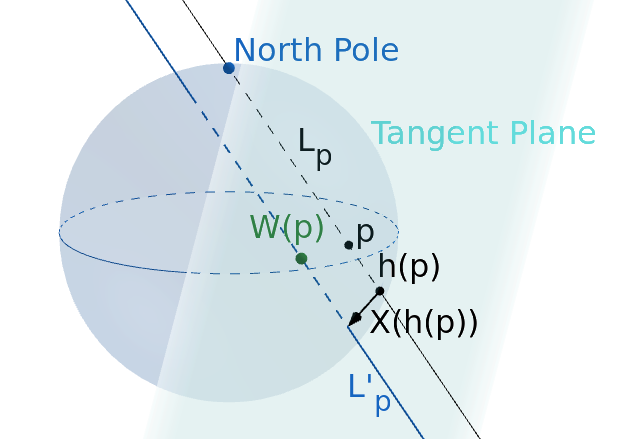
\includegraphics[scale=.4]{HairyBallW.png}
	\end{figure}

	Since $X$ is a non-vanishing continuous vector field, $W\colon \bbD^{2}\to \R^{2}$ is a non-vanishing continuous function.
	Therefore it induces a continuous function
	\begin{align*}
	    F\colon \bbD^{2} &\longrightarrow \bbS^{1} \\
	    p &\longmapsto \frac{F(p)}{|F(p)|}.
	\end{align*}
	We repeat the same process with the south pole and $\bbS^{2}_{+}$.
	This gives us a non-vanishing continuous function $W^{*}\colon \bbD^{2}\to \R^{2}$ that we can again normalise into a continuous function $F^{*}\colon \bbD^{2}\to \bbS^{1}$.

	We denote by $f$ and $f^{*}$ the restrictions to $\bbS^{1}\subseteq \bbD^{2}$ of $F$ and $F^{*}$ respectively.
	By definition $f$ and $f^{*}$ factor through the contractible space $\bbD^{2}$:
	\begin{center}
	    \begin{tikzcd}
		\bbS^{1}\arrow[hook]{dr} \arrow{rr}{f,f^{*}} & & \bbS^{1} \\
		 & \bbD^{2}\arrow[swap]{ur}{F,F^{*}} &
	    \end{tikzcd}
	\end{center}
	Therefore, they are both nullhomotopic.

	To obtain the desired contradiction, we will next find a certain relation between the functions $f$ and $f^{*}$, which is in turn induced by a relation between $W|_{\bbS^{1}}$ and $W^{*}|_{\bbS^{1}}$.
	Namely, given a point $p=h(p)=(x_{0},y_{0},0)\in \bbS^{1}\subseteq \bbD^{2}$, we claim that
	\begin{equation}
	    W^{*}(p)=R_{p}(W(p)).
	\end{equation}
	Recall that this means that the vector $W^{*}(p)$ is the linear reflection of $W(p)$ across the axis given by the direction defined by $(-y_{0},x_{0},0)\in \R^{2}$.
	In order to prove this, we fix an arbitrary $p=(x_{0},y_{0},0)\in \bbS^{1}$ and we change the coordinate system, making $p$ the origin, $(x_{0},y_{0},0)$ the first basis vector in $\R^{2}$ and $(-y_{0},x_{0},0)$ the second basis vector in $\R^{2}$.
	We express $W(p)$ and $W^{*}(p)$ with respect to these coordinates:
	\[ W(p)=(w_{1},w_{2},0) \text{ and } W^{*}(p)=(w_{1}^{*},w_{2}^{*},0). \]
	The claim is then that $w_{1}=-w_{1}^{*}$ and $w_{2}=w_{2}^{*}$.

	We check first that $w_{2}=w_{2}^{*}$.
	Let $L_{p}$ resp.~$L_{p}^{*}$ denote the line joining $p$ to the north resp.~south pole.
	These two lines intersect at $p$ and define a plane $\Pi$ which intersects $\R^{2}$ precisely along the $x$-axis of our current coordinate system.
	Let $L_{p}'$ resp.~$(L_{p}^{*})'$ be the lines with directions equal to those of $L_{p}$ resp.~$L_{p}^{*}$ containing the point $p+X(p)$.
	The plane $\Pi'$ defined by these two lines is then parallel to $\Pi$, and therefore the intersection $\Pi'\cap \R^{2}$ is parallel to the $x$-axis of our current coordinate system.
	This implies that $w_{2}=w_{2}^{*}$.

	To check that $w_{1}=w_{1}^{*}$ we argue projecting the whole picture into the plane spanned by the vectors $(x_{0},y_{0},0)$ and $(0,0,1)$.
	From this point of view we see the following picture:
	
	\begin{figure}[htp]
	    \centering
	    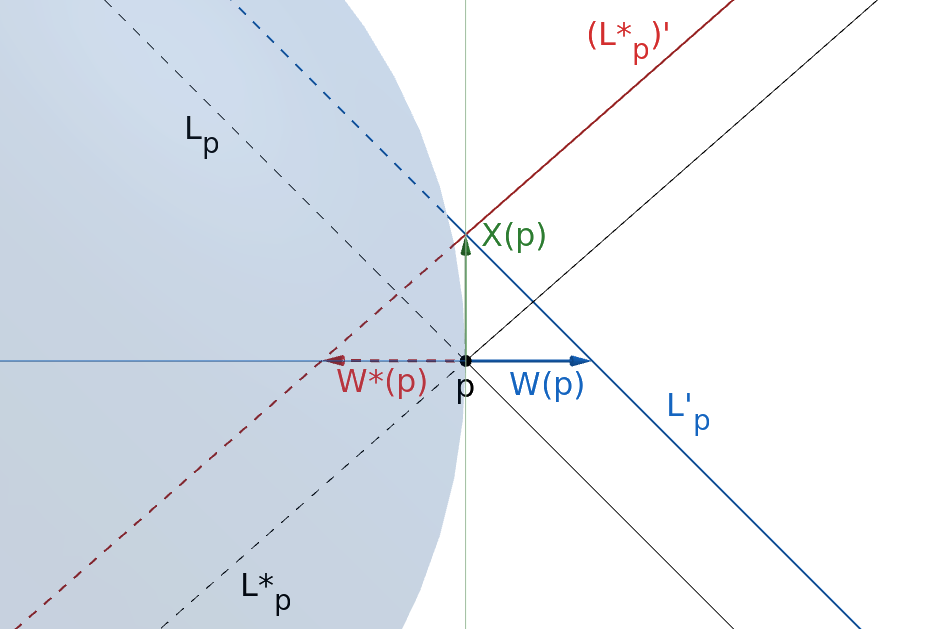
\includegraphics[scale=.4]{HairyBall1.png}
	\end{figure}

	From Thales' theorem we know that $L_{p}$ and $L^{*}_{p}$ intersect at a right angle.
	From Proposition $29$ in Book I of Euclid's \textit{Elements} we deduce that all other angles that seem to be right angles in the picture are in fact right angles.
	From the fact that the inner angles of any triangle add up to two right angles we deduce in turn that all angles that look like half a right angle in the picture are in fact half a right angle.
	Indeed, we can start by ensuring that the inner angle between $L_{p}$ and $W^{*}(p)$ is half a right angle, which follows from the fact that the triangle with vertices $p$, the usual origin of $\R^{3}$ and the north pole is isosceles with a right angle at the usual origin of $\R^{3}$.
	Then, knowing already that the inner angle between $W^{*}(p)$ and $X(p)$ is a right angle, we deduce from this that the inner angle between $L_{p}$ and $X(p)$ is also half a right angle, and so on.
	This implies that all four small triangles in the picture are congruent, and in particular $w_{1}=w_{1}^{*}$.

	We are finally ready to exhibit the desired contradiction.
	Let $H\colon \bbS^{1}\times [0,1]\to \bbS^{1}$ be a homotopy from $f$ to the constant map $c\colon \bbS^{1}\to \bbS^{1}$ with constant value the poitn $(-1,0,0)\in \bbS^{1}\subseteq \R^{3}$.
	The formula
	\begin{align*}
	    H^{*}\colon \bbS^{1}\times [0,1] & \longrightarrow \bbS^{1} \\
	    (p,t) & \longmapsto R_{p}(H(p,t))
	\end{align*}
	defines a homotopy between the nullhomotopic map $f^{*}\colon \bbS^{1}\to \bbS^{1}$ and the map
	\begin{align*}
	    c^{*}\colon \bbS^{1} & \longrightarrow \bbS^{1} \\
	    p  & \longmapsto R_{p}((-1,0,0))
	\end{align*}
	But this is a contradiction, because $c^{*}\colon \bbS^{1}\to \bbS^{1}$ is the morphism going twice around $\bbS^{1}$ at constant speed and starting from $(1,0,0)$, which is not nullhomotopic.
    \end{proof}
\end{thm}

If we take the Whitney embedding theorem \cite[Theorem II.10.7]{bre93}, the tubular neighbourhood theorem \cite[Theorem II.11.4]{bre93} and the Lefschetz--Hopf fixed point theorem \cite[Theorem IV.23.4]{bre93} for granted, we can prove a much more general statement:

\begin{thm}[{\cite[Corollary IV.23.6]{bre93}}]
    If $M$ is a compact smooth manifold with Euler characteristic $\chi(M)\neq 0$, then any continuous vector field on $M$ has a zero.
    \begin{proof}
	We show that if $M$ admits a non-vanishing continuous vector field, then it has Euler characteristic $\chi(M)=0$.
	So let $X\colon M\to TM$ be a non-vanishing continuous vector field on $M$.

	The Whitney embedding theorem \cite[Theorem II.10.7]{bre93} allows us to assume that $M\subseteq \R^{N}$ is a compact smooth submanifold.
	The tubular neighbourhood theorem \cite[Theorem II.11.4]{bre93} ensures the existence of a small enough real number $\varepsilon >0$ such that the sum in $\R^{N}$ yields a diffeomorphism
	\[ \theta\colon \{ (x,v)\in M\times \R^{N}\mid v\perp T_{x}M, \lVert v \rVert<\varepsilon \} \cong \{ y\in \R^{N}\mid \operatorname{dist}(M,y)<\varepsilon\} \]
	from the open subset $N_{\varepsilon}M$ of the normal bundle consisting of normal vectors with norm less than $\varepsilon$ to an $\varepsilon$-neighbourhood $B_{\varepsilon}M$ of $M$ in $\R^{N}$, which we refer to as a \textit{tubular neighbourhood} of $M$ in $\R^{N}$.
	The projection from the normal bundle $\pi\colon NM\to M$ induces a smooth strong deformation retraction $r\colon B_{\varepsilon}M\to M\subseteq B_{\varepsilon}M$ given by $y\mapsto \pi(\theta^{-1}(y))$.
	The smooth homotopy that shows that $r$ is a smooth strong deformation retraction \cite[Definition I.14.8]{bre93} is
	\begin{align*}
	    F\colon B_{\varepsilon}M\times [0,1] & \longrightarrow B_{\varepsilon}M \\
	    (\theta(x,v),t) & \longmapsto \theta(x,tv)
	\end{align*}
	Since $M$ is compact, we may assume ---up to multiplying $X$ by a small enough scalar--- that $\lVert X(x) \rVert<\varepsilon$ for all $x\in M$.
	We define then
	\begin{align*}
	    f\colon M &\longrightarrow M\\
	    x &\longmapsto r(x+X(x)).
	\end{align*}
	Geometrically, we are projecting the point $x+X(x)\in \R^{N}$ onto $M$ along the normal direction:

	\todo{figure}

	If $f(x)=x$, then the tangent direction of $X(x)$ is zero.
	But $X(x)$ was by assumption a tangent vector at $x\in M$, so $X(x)=0$, contradicting the assumption that $X$ is non-vanishing.
	Thus $f$ has no fixed points.

	We have also shown as a consequence of the Whitney embedding theorem that $M$ is an euclidean neighbourhood retract.
	Namely, $M$ is a retract of the open subset $B_{\varepsilon}M\subseteq \R^{N}$.
	Therefore we may apply the Lefschetz--Hopf fixed point theorem \cite[Corollary IV.23.5]{bre93} to deduce that
    \end{proof}
\end{thm}

\bibliographystyle{alpha}
\bibliography{main}
\vfill

\end{document}

